\documentclass{article}
\usepackage{graphicx}
\usepackage{amsmath}
\usepackage[margin=1in]{geometry}
\usepackage{array}
\usepackage{listings}
\usepackage{xcolor}
\usepackage{tikz}
\usetikzlibrary{arrows}

\setlength{\parindent}{0pt}

\definecolor{codegreen}{rgb}{0,0.6,0}
\definecolor{codegray}{rgb}{0.5,0.5,0.5}
\definecolor{codepurple}{rgb}{0.58,0,0.82}
\definecolor{backcolour}{rgb}{0.95,0.95,0.92}

\lstdefinestyle{mystyle}{
	language=Java,
    backgroundcolor=\color{backcolour},
    commentstyle=\color{codegreen},
    keywordstyle=\color{blue},
    numberstyle=\tiny\color{codegray},
    stringstyle=\color{codepurple},
    basicstyle=\ttfamily,
    breakatwhitespace=false,
    breaklines=true,
    captionpos=b,
    keepspaces=true,
    numbers=left,
    numbersep=5pt,
    showspaces=false,
    showstringspaces=false,
    showtabs=false,
    tabsize=2
}

\lstset{style=mystyle}

\title{3S03 A2}
\author{Matthew Nesbitt, nesbim2, 400463297}
\date{February 2025}

\begin{document}
\maketitle
\section{Question 1}
\subsection{Part A}
There are two bugs I found in RomanNumerals. These bugs were identified using visual static analysis by reading through the code. I then
confirmed the bugs I had identified by running testcases that would exploit those faults to cause faulty output.
Firstly, an input of 9 results in "IVX", due to the final line in \lstinline{romanForDigit()} of
\lstinline{return "" + one + five + ten;}. This would be fixed by modifying this line to be \lstinline{return "" + one + ten;}. Secondly, There
is missing functionality for numbers beyond 9, where the values will begin wrapping back around to 0. This would be fixed by modifying the
line \lstinline{return romanForDigit(i, 'I', 'V', 'X');} to support the tens column by re-using the \lstinline{romanForDigit()} function
with different symbols: \lstinline{return romanForDigit(x, 'X', 'L', 'C') + romanForDigit(i, 'I', 'V', 'X');},
which would allow RomanNumerals to support input $0 \leq x \leq 99$.
\subsection{Part B}
Tests available in q1.zip.\\
Test run success:\medskip \\
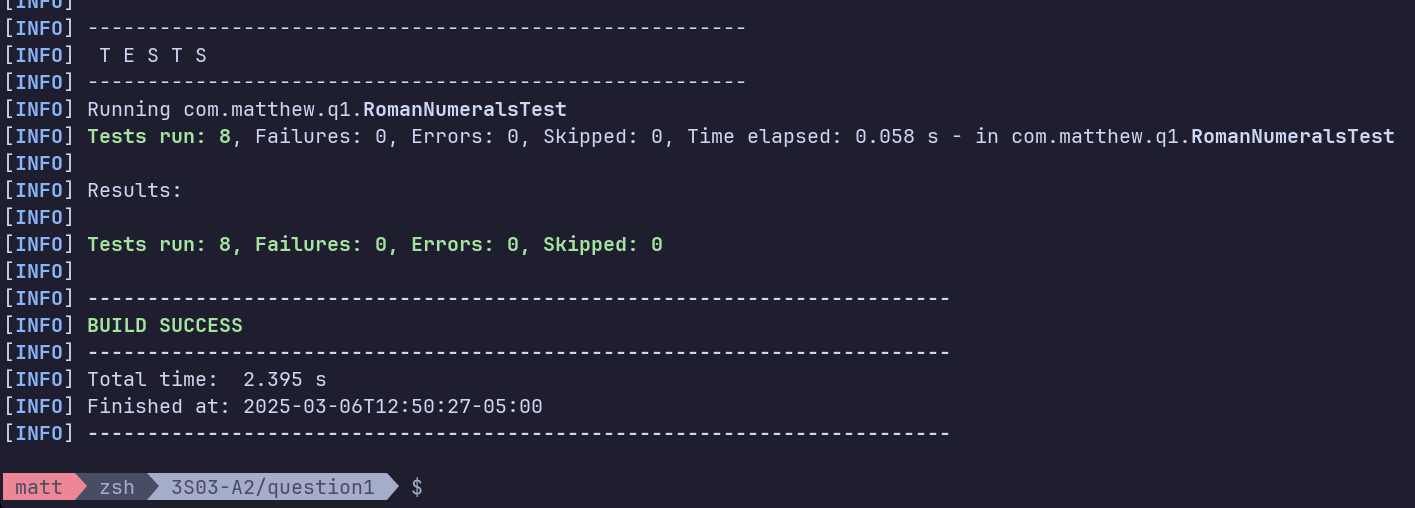
\includegraphics[scale=0.3]{tests.png}
\subsection{Part C}
A screenshot from SonarQube showing 100\% statement and 100\% condition coverage:\\
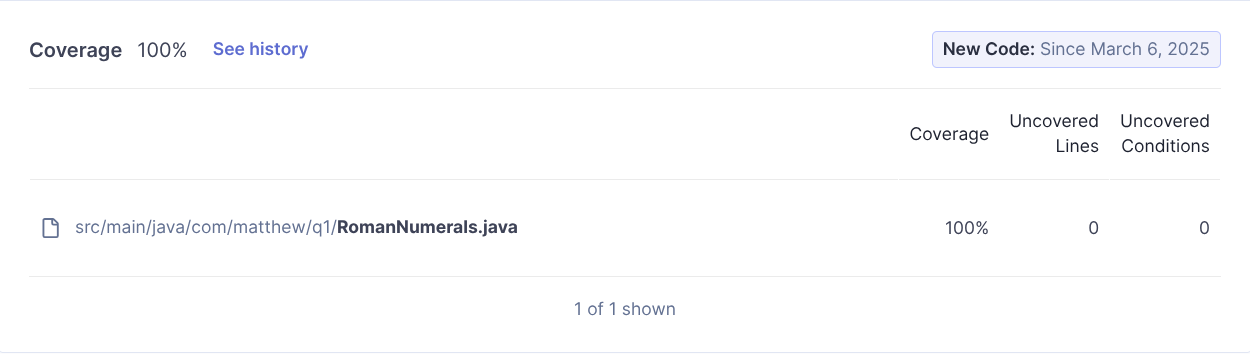
\includegraphics[scale=0.3]{sonarq.png}\\
A screenshot from the JaCoCo output file showing 100\% branch coverage:\\
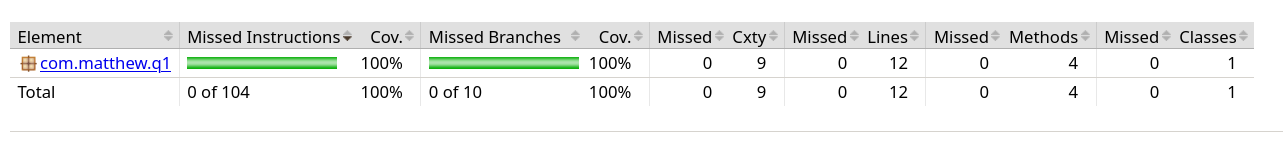
\includegraphics[scale=0.3]{jacoco.png}\\
My test suite also has 100\% MC/DC coverage as it meets all 4 required criteria:
\begin{itemize}
	\item 1: 100\% branch converage (shown in JaCoCo)
	\item 2: 100\% condition converage (shown in SonarQube)
	\item 3: As the only module is RomanNumerals, we cover the only entry point (RomanNumerals.roman()) as well as the only exit point
		(RomanNumerals.roman()).
	\item 4: Since every if statement only has one condition, a change in that condition \textit{must} independently affect the output.
		Due to this, exercising every condition (condition converage) implies condition 4 for MC/DC.
\end{itemize}
\end{document}
